In this section we derive the coefficients (\ref{eq:expansion_coefficients_debye_BCF_SBM_Matsubara}) and (\ref{eq:expansion_coefficients_debye_BCF_SBM_Pade}) that can be used to approximate the bath correlation function
\begin{equation*}
    \alpha(\tau) = \frac{1}{\pi} \int_0^\infty S(\omega)
    \left[
        \coth\left(\frac{\omega}{2T}\right)\cos(\omega\tau)-i\sin(\omega\tau)
    \right]\text{d}\omega
    = \int_0^\infty I(\omega,\tau)\text{d}\omega
\end{equation*}
with the \textit{Debye spectral density}
\begin{equation*}
    S(\omega) = \eta \frac{\omega\gamma}{\omega^2+\gamma^2}
\end{equation*}
as a sum of exponentials
\begin{equation*}
    \alpha(\tau) \approx \sum_{k=0}^{K-1}g_ke^{-\omega_k\tau}.
\end{equation*}
We first note that the integrand $I(\omega, \tau)$ is symmetric with respect to $\omega$; $\,I(-\omega, \tau) = I(\omega, \tau)$.
Therefore, we can extend the integral over the negative real axis:
\begin{equation*}
    \alpha(\tau) = \frac{1}{2\pi} \int_{-\infty}^\infty S(\omega)
    \left[
        \coth\left(\frac{\omega}{2T}\right)\cos(\omega\tau)-i\sin(\omega\tau)
    \right]\text{d}\omega.
\end{equation*}
Next, we write the sine and cosine in terms of complex exponentials and use the identity $\coth(x) = 2f^\text{Bose}(2x) - 1$
with the \textit{Bose function}
\begin{equation*}
    f^\text{Bose}(x) \coloneqq \frac{1}{1-e^{-x}}
\end{equation*}
to arrive at
\begin{equation}
    \label{eq:transformed_BCF_Bose}
    \alpha(\tau) = \frac{1}{\pi} \int_{-\infty}^\infty S(\omega)
    \left[
        f^\text{Bose}(\omega\beta)-1
    \right]\text{d}\omega.
\end{equation}
In the following, we will derive two different approximations of this integral.

\subsection*{Matsubara frequency summation}
The Matsubara frequency summation uses the residue theorem to turn the integral (\ref{eq:transformed_BCF_Bose}) into an infinite
sum. This sum then has to be truncated to get an approximation with a finite number of terms. The resulting approximation works well at high temperatures,
but converges only slowly at low temperatures.\\
Consider the line integral in Figure \ref{fig:line_integral_matsubara_expansion}. Because of the exponential term
$e^{i\omega\tau}$, the contribution along $L_2$ vanishes as we take the limit $R \rightarrow \infty$. This then leaves us with
\begin{equation*}
    \begin{split}
        \alpha(\tau) &= \frac{1}{\pi} \oint_\xi S(\omega) \left[
            f^\text{Bose}(\omega\beta)-1
        \right]\text{d}\omega = 2i \sum_{\{\omega_j\}}\Res\left(
            S(\omega)e^{-i\omega\tau}\left[
            f^\text{Bose}(\omega\beta)-1
            \right]; \omega_j\right) \\
            &= 2i \sum_{\{\omega_j^\prime\}} \Res\left(
                S(\omega); \omega_j^\prime
            \right) e^{i\omega_j^\prime\tau} \left[ f^\text{Bose}(\omega_j^\prime\beta)-1 \right]
            + 2i\sum_{\{\omega_j^{\prime\prime}\}}\Re\left(
                f^\text{Bose}(\omega\beta); \omega_j^{\prime\prime}
            \right) S(\omega_j^{\prime\prime}) e^{i\omega_j^{\prime\prime}\tau},
    \end{split}
\end{equation*}
where $\omega_j$ are the poles of $S(\omega) \left[f^\text{Bose}(\omega\beta)-1\right]$, $\omega_j^\prime$ the poles of
$S(\omega)$, $\omega_j^{\prime\prime}$ the poles of $f^\text{Bose}(\omega\beta)$, and we have used the residue theorem.
We also assumed that
$\omega_i^\prime \neq \omega_j^{\prime\prime}$ for all $i, j$, which is the case for almost all $\gamma, \beta$.
Next, we need to compute all poles and residues. The Debye spectral density has simple poles at $\omega_j^\prime=\pm i\gamma$,
with residues
\begin{equation*}
    \Residue\left(S(\omega);\pm i\gamma\right) = \lim_{\omega\rightarrow i\gamma}(\omega\mp i\gamma)S(\omega) = \frac{\eta\gamma}{2}.
\end{equation*}
The poles of the Bose function lie on the imaginary axis, $\omega_j^{\prime\prime} = 2\pi in/\beta$ with $n\in\mathbb{Z}$,
and are again simple poles with residues
\begin{equation*}
    \Re\left(
        f^\text{Bose}(\omega\beta); \frac{2\pi in}{\beta}
    \right) = \lim_{\omega \rightarrow 2\pi in/\beta} \frac{(\omega-2\pi in/\beta)}{1-e^{-\omega\beta}} =
    \lim_{x\rightarrow0}\frac{x}{1-e^{-\beta x-2\pi i n}} = \lim_{x\rightarrow0} \frac{1}{\beta e^{-\beta x}} = \frac{1}{\beta},
\end{equation*}
where we substituted $x = \omega - 2\pi i n/\beta$ and used the rule of L'Hopital.\\
With this, we are now equipped to solve the integral:
\begin{equation*}
    \alpha(\tau) = \frac{\eta\gamma}{2} e^{-\gamma\tau}\left[\cot(\gamma\beta)-i\right]e^{-\gamma\tau}
    + \sum_{k=1}^{\infty} \eta\frac{4\pi T^2k\gamma}{4\pi^2T^2k^2-\gamma^2} e^{-2\pi Tk\tau} = \sum_{k=0}^{\infty} g_ke^{-\omega_k\tau}
\end{equation*}
with the coefficients (\ref{eq:expansion_coefficients_debye_BCF_SBM_Matsubara}).
The result is similar to the one obtained in \cite{Qiang:2009} (up to a different normalization).
  
\subsection*{Padé spectrum decomposition}
The Padé spectrum decomposition is a method to approximate the Bose function $f_\text{Bose}(x)$ by a finite sum \cite{Hu:2011}. We will use the Padé approximant
$[N-1/N]$ with $N\equiv K-1$ to rewrite
\begin{equation*}
    \alpha(\tau) \approx \frac{1}{\pi} \int_{-\infty}^{\infty} S(\omega) e^{i\omega\tau}
    \left[
        \frac{1}{\omega\beta}-\frac{1}{2}+\sum_{k=1}^{K-1}\frac{2\tilde{\eta}_k\omega_\beta}{(\omega\beta)^2+\tilde{\xi}_k^2}
    \right]\text{d}\omega,
\end{equation*}
where the derivation of the constants $\tilde{\eta}_k$ and $\tilde{\xi}_k$ can be found in \cite{Hu:2011}.
We can now proceed in a similar way to the Matsubara frequency summation. We will again consider the line integral along
the contour in Figure \ref{fig:line_integral_matsubara_expansion} and use the residue theorem. The poles and residues of the
new terms are
\begin{equation*}
    \Res\left(
        \frac{1}{\omega\beta}; 0
    \right) = \frac{1}{\beta}
\end{equation*} 
and
\begin{equation*}
    \Res\left(
        \frac{2\tilde{\eta}_k\omega\beta}{(\omega\beta)^2+\tilde{\xi}_k^2}; \pm i\frac{\tilde{\xi}_k}{\beta}
    \right) = \frac{\tilde{\eta}_k}{\beta}.
\end{equation*}
A bit of algebra yields the final result
\begin{equation*}
    \alpha(\tau) \approx \eta\gamma\left[
        \frac{1}{\gamma\beta}-\frac{i}{2}-\sum_{k=1}^{K-1}\frac{2\tilde{\eta}_k\gamma\beta}{\tilde{\xi}_k^2-\gamma^2\beta^2}
    \right] e^{-\gamma\tau}
    + \sum_{k=1}^{K-1} \frac{2\tilde{\eta}_k\eta\gamma\tilde{\xi}_k}{\tilde{\xi}_k^2-\gamma^2\beta^2} e^{-\frac{\tilde{\xi}_k}{\beta}\tau}
    = \sum_{k=0}^{K-1}g_ke^{-\omega_k\tau}
\end{equation*}
with the coefficients (\ref{eq:expansion_coefficients_debye_BCF_SBM_Pade}).
\begin{figure}[!ht]
    \centering
    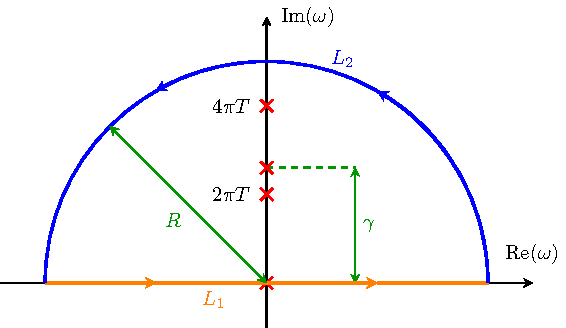
\includegraphics{tikz/matsubara_expansion/matsubara_expansion.pdf}
    \caption[short]{In this figure, the line integral for computing the expansion of the bath correlation function is shown.}
    \label[figure]{fig:line_integral_matsubara_expansion}
\end{figure}